\subsection{Exemple d'équation}
  \begin{align}
    V = RI \\
    V = RI \\
    V = RI
  \end{align}

\subsection{Exemple de tableau}
  \begin{table}[H]
    \begin{center}
      \caption{Exemple de tableau}
      \begin{tabular}{L{4cm} L{4cm} L{4cm}} 
        \hline
        \textbf{Colonne 1} & \textbf{Colonne 2} & \textbf{Colonne 3} \\ [0.75ex] 
        \hline\hline
        Ligne 1 & & \\
        Ligne 2 & & \\
        Ligne 3 & & \\
        Ligne 4 & & \\
        Ligne 5 & & \\ [1ex]
        \hline
      \end{tabular}
    \end{center}
  \end{table}

\subsection{Exemple de graphique}
  \begin{figure}[H]
    \centering
    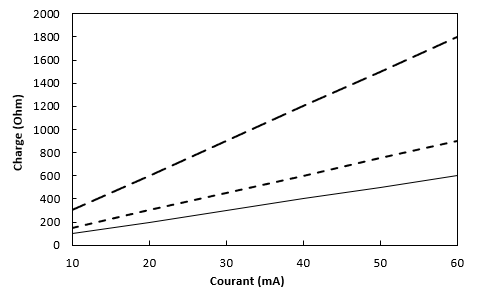
\includegraphics[scale=1]{Images/Graph.png}
    \caption{Exemple de graphique}
    \label{fig:Graph}
  \end{figure}

\subsection{Exemple d'histogramme}
  \begin{figure}[H]
    \centering
    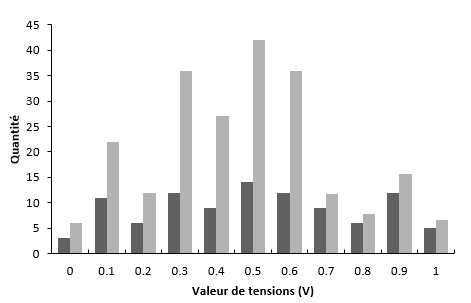
\includegraphics[scale=1]{Images/Histogram.png}
    \caption{Exemple d'histogramme}
    \label{fig:Histogram}
  \end{figure}
